% Codex-assisted presentation document, not application/test source.
% XeLaTeX. Theme provenance and rights: template-provenance.json and NOTICE.md.
\documentclass[aspectratio=169,11pt,t]{beamer}
\PassOptionsToPackage{no-math}{fontspec}
\usepackage[UTF8,fontset=fandol]{ctex}
\defaultfontfeatures{Path=fonts/}
\usetheme[sectionpages=false]{CityU}
\defaultfontfeatures{}
\usepackage{booktabs,tabularx,amsmath}
\usetikzlibrary{arrows.meta,positioning}
\setbeameroption{hide notes}
% Match the physical PDF pages used in the bilingual notes index.
\addtobeamertemplate{footline}{%
  \begingroup
  \def\insertframenumber{\thepage}%
  \def\inserttotalframenumber{\insertdocumentendpage}%
}{\endgroup}
\setlength{\tabcolsep}{5pt}
\newcolumntype{L}[1]{>{\raggedright\arraybackslash}p{#1}}
\newcolumntype{Y}{>{\raggedright\arraybackslash}X}
\newcommand{\source}[1]{\par\vfill{\fontsize{6.6}{8}\selectfont\color{CityUMuted}Source: #1\par}}
\newcommand{\takeaway}[1]{\par\medskip{\color{CityUTeal}\bfseries #1\par}}
\newcommand{\code}[1]{{\ttfamily\small #1}}
\title[EvidenceGuard]{EvidenceGuard\\TradingAgents}
\subtitle{Deterministic evidence and release checks}
\author{Group 42}
\institute{CS5351 Software Engineering, City University of Hong Kong}
\date{Evidence snapshot: 20 November 2026}
\cityufooter{EvidenceGuard \quad CS5351 \quad Group 42 \quad Status: 20 Nov 2026}
\begin{document}
\cityutitlepage

\begin{frame}{Research problem and scope}
 A persuasive stock report can still contain references that are difficult to audit.
 \medskip
 \begin{itemize}\setlength\itemsep{6pt}
  \item Was the source available at the analysis cutoff?
  \item Does each factual claim identify eligible evidence?
  \item Do retries stay within the run and project budgets?
  \item Has a person approved this exact report revision?
 \end{itemize}
 \takeaway{Initial scope: AAPL, MSFT and NVDA, with market and news analysts}
 \small One investment debate round and one risk debate round. Local research only.
 \source{Report.md, sections 1 and 3; Blueprint.md}
\end{frame}

\begin{frame}{Upstream reuse and extension}
 \small
 \begin{tabularx}{\textwidth}{@{}L{.43\textwidth}Y@{}}
 \toprule\textbf{TradingAgents already provides}&\textbf{EvidenceGuard adds}\\\midrule
 Analysts, investment debate and risk debate & Evidence IDs, source times and content hashes\\[5pt]
 Structured decisions and plain-text fallback & Claim references and an independent final gate\\[5pt]
 Model settings and token statistics & Request reservation, settlement and stopping\\[5pt]
 CLI and report generation & Replay, paired evaluation and hash-bound review\\\bottomrule
 \end{tabularx}
 \medskip\normalsize Upstream license, layout and historical tests remain in place.
 \par\small Extension: \code{src/evidenceguard/}; optional upstream graph boundary.
 \source{docs/req/baseline-review.md; Report.md, section 2. Upstream SHA: 9fa1196fffbcfd9de5146d2dd2869df84ab99838}
\end{frame}

\begin{frame}{Seven functional requirements}
 \small
 \begin{tabularx}{\textwidth}{@{}L{1.5cm}L{3.7cm}Y@{}}
 \toprule ID&Capability&Observable result\\\midrule
 FR-001&Frozen run contract&Versioned inputs and analysis cutoff\\
 FR-002&Evidence qualification&Eligible and excluded evidence retained\\
 FR-003&Claim and conflict cards&References within the same run\\
 FR-004&Independent validation&Violations block progression\\
 FR-005&Request budgets&Reserved, settled, unknown or stopped\\
 FR-006&Replay and evaluation&Frozen plan, failures and usage retained\\
 FR-007&Human review&Approval bound to the current hash\\\bottomrule
 \end{tabularx}
 \takeaway{Component implementation exists. Full protocol acceptance remains incomplete.}
 \source{docs/req/requirements.yaml; docs/architecture/trace-matrix.md; v0.3/final-review.md}
\end{frame}

\begin{frame}{Architecture and decision authority}
 \centering
 \begin{tikzpicture}[node distance=5mm and 5mm,box/.style={draw=CityUTeal,rounded corners=1mm,align=center,font=\small,minimum height=10mm,text width=25mm,inner sep=3pt},arr/.style={-{Latex[length=2mm]},thick,draw=CityUMuted}]
 \node[box] (contract) {Frozen\\contract};
 \node[box,right=of contract] (ledger) {Evidence\\ledger};
 \node[box,right=of ledger] (graph) {Upstream graph\\and claim turns};
 \node[box,right=of graph] (gate) {Independent\\final gate};
 \node[box,below=12mm of gate] (draft) {Draft artifact};
 \node[box,left=of draft] (human) {Human review\\of current hash};
 \node[box,left=of human] (release) {Publication\\recheck};
 \node[box,left=of release] (budget) {Request budget\\ledger};
 \draw[arr] (contract)--(ledger);\draw[arr] (ledger)--(graph);\draw[arr] (graph)--(gate);
 \draw[arr] (gate)--(draft);\draw[arr] (draft)--(human);\draw[arr] (human)--(release);
 \draw[arr,dashed] (budget.north east)--(graph.south);
 \end{tikzpicture}
 \par\medskip\raggedright
 \textbf{LLM:} proposes claims, inferences and conflicts.\par
 \textbf{Code:} validates eligibility, references, budgets and release conditions.\par
 \textbf{Student:} reviews semantic support and makes genuine approval decisions.
 \source{Blueprint.md; docs/architecture/interface-contracts.md; Report.md, section 3}
\end{frame}

\begin{frame}{Evidence time and context}
 \begin{columns}[T,onlytextwidth]
 \begin{column}{.49\textwidth}
 \textbf{Qualification rule}\medskip
 \begin{itemize}\setlength\itemsep{5pt}
 \item Market: \code{available\_at}
 \item News: \code{published\_at}
 \item Compare source time with cutoff
 \item Keep unknown or future sources as excluded
 \end{itemize}
 \end{column}
 \begin{column}{.47\textwidth}
 \textbf{v0.3 context contract}\medskip
 \begin{itemize}\setlength\itemsep{5pt}
 \item At most one market record
 \item At most three news records
 \item Stable time and ID ordering
 \item Full ledger and missing-data notes remain
 \end{itemize}
 \end{column}
 \end{columns}
 \takeaway{Retrieval time cannot establish when information became available.}
 \source{docs/architecture/interface-contracts.md; docs/verification/v0.3/final-review.md}
\end{frame}

\begin{frame}{Artifact state and human review}
 \small
 \begin{tabularx}{\textwidth}{@{}L{2.9cm}L{3.2cm}Y@{}}
 \toprule Axis&Example values&Meaning\\\midrule
 Execution&completed / failed&Did the run finish?\\
 Validation&passed / failed&Did independent checks pass?\\
 Review&pending / approved&Did a person review this hash?\\
 Publication&draft / released&Did publication recheck succeed?\\\bottomrule
 \end{tabularx}
 \medskip\normalsize
 \[\text{release}\Rightarrow\text{completed}\land\text{gate passed}\land\text{approval of current hash}\]
 Business content changes produce a new hash and invalidate the old approval.
 \source{src/evidenceguard/review.py; docs/architecture/interface-contracts.md}
\end{frame}

\begin{frame}{Request budgets}
 \begin{itemize}\setlength\itemsep{7pt}
 \item Reserve a conservative bound before every HTTP request.
 \item Count retries, repair and auxiliary requests.
 \item Settle known usage. Retain reservations when usage is unknown.
 \item Stop generation when a boundary rejects the request.
 \end{itemize}
 \medskip
 Project ceiling: \textbf{USD95}. Development: USD55. Application and reserve: USD40.
 \takeaway{All 200 development requests had been used at the evidence cutoff.}
 \small The request count and dollar cap are enforced separately.
 \source{v0.3/final-review.md; docs/pending-actions.md. Recorded development request count}
\end{frame}

\begin{frame}{FR-007 traceability}
 \small
 \begin{tabularx}{\textwidth}{@{}L{2.8cm}Y@{}}
 \toprule Artifact&FR-007: current-hash approval\\\midrule
 Requirement&A changed report cannot reuse a previous approval.\\[4pt]
 Design&Canonical business projection and SHA-256 hash.\\[4pt]
 Implementation&\code{review.artifact\_hash} and publication recheck.\\[4pt]
 Negative case&Change business content after review, then attempt publication.\\[4pt]
 Expected&Hash mismatch or missing current approval rejects publication.\\[4pt]
 Evidence&\code{test\_gate\_review.py} and regression logs.\\\bottomrule
 \end{tabularx}
 \takeaway{Expected outcomes follow the contract, independently of model output.}
 \source{docs/architecture/trace-matrix.md; interface-contracts.md; src/evidenceguard/review.py; offline tests}
\end{frame}

\begin{frame}{Research workbench}
 \begin{columns}[T,onlytextwidth]
 \begin{column}{.68\textwidth}
 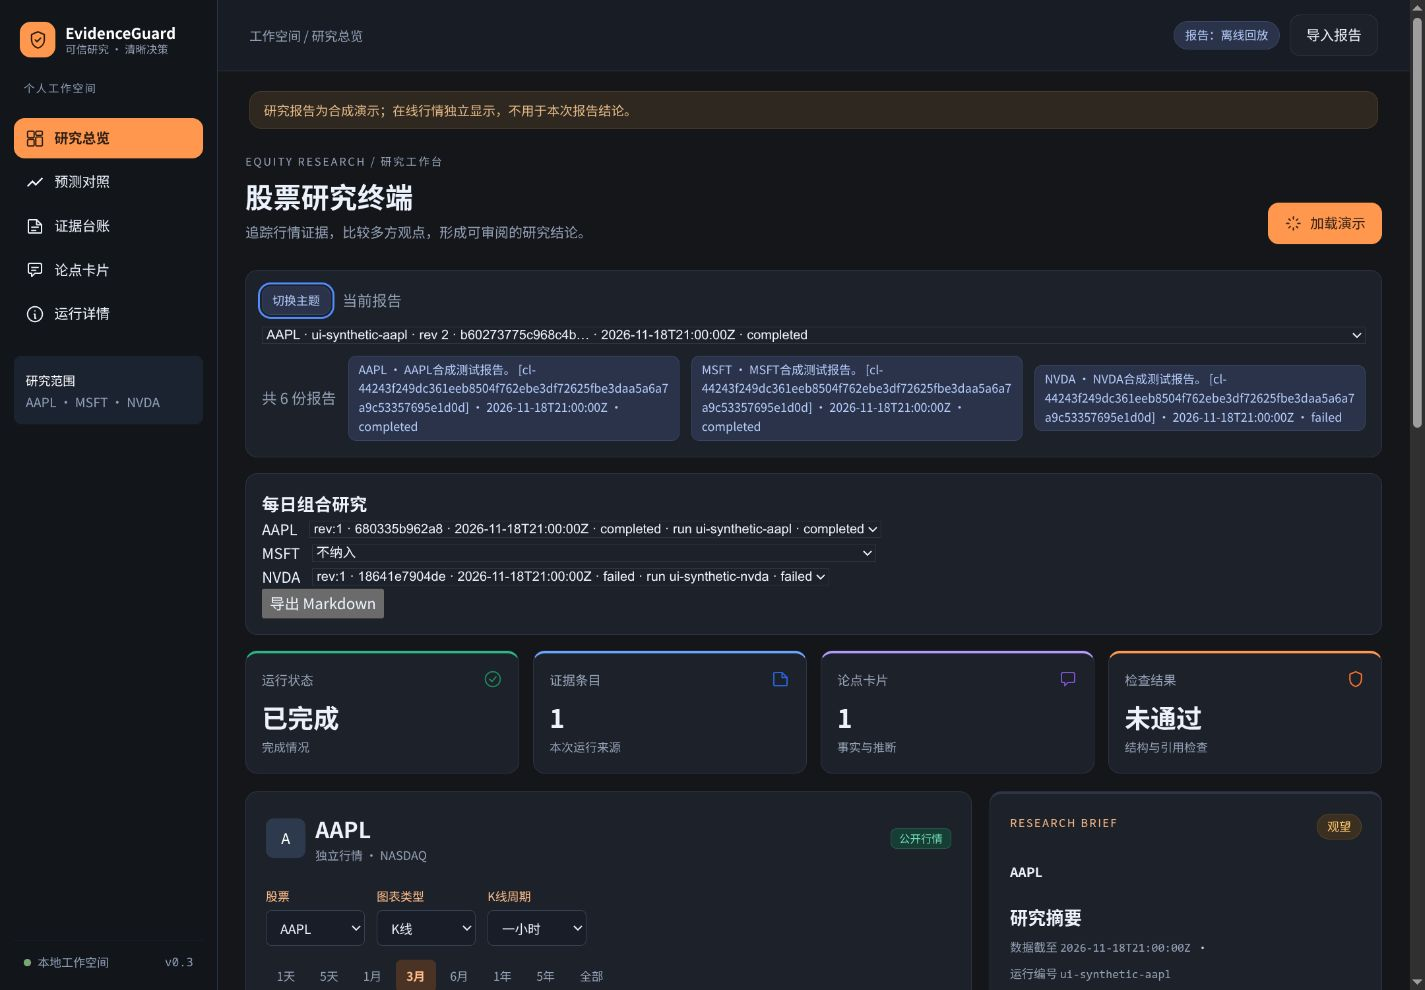
\includegraphics[width=\linewidth,height=4.75cm,keepaspectratio]{figures/desktop-dark-top.jpg}
 \end{column}
 \begin{column}{.29\textwidth}\small
 Manual import\par\medskip Report revisions\par\medskip Claim references\par\medskip
 Source details\par\medskip Markdown and JSON export
 \end{column}
 \end{columns}
 \medskip\small\alert{Actual browser QA with synthetic fixtures. Business quality remains unmeasured.}
 \source{docs/verification/v0.3/screenshots/desktop-dark-top.jpg; final-review.md, browser QA}
\end{frame}

\begin{frame}{Offline demonstration}
 \begin{enumerate}\setlength\itemsep{8pt}
 \item Replay the existing synthetic fixture.
 \item Inspect evidence times, claim references and the report.
 \item Show \textbf{completed / passed / pending / draft}.
 \item Attempt publication without approval and observe rejection.
 \end{enumerate}
 \takeaway{Deterministic replay uses zero model requests.}
 \small Fixture version identity is a placeholder. This is separate from formal evaluation.
 \source{examples/offline-replay.json; src/evidenceguard/\_\_main\_\_.py; v0.3/public-regression.txt}
\end{frame}

\begin{frame}{Verification evidence and its limits}
 \small
 \begin{tabularx}{\textwidth}{@{}L{3.0cm}L{3.1cm}Y@{}}
 \toprule Check&Recorded result&Scope\\\midrule
 Offline regression&1687 passed&Rerun on 20 Nov, 1 skip and 1 deselection\\[4pt]
 Ruff and JS syntax&Passed&Prior archived run, seven JS scripts\\[4pt]
 Browser QA&Desktop and phone&Real UI operations, synthetic fixtures\\[4pt]
 Gate benchmark&p95 1.069 ms&Synthetic 100 claims, 25 evidence records\\[4pt]
 Business evaluation&Pending&No measured quality or token-saving result\\\bottomrule
 \end{tabularx}
 \takeaway{Passing regression does not establish complete v0.3 acceptance.}
 \source{docs/verification/v0.3/final-review.md; docs/verification/gate-performance.json}
\end{frame}

\begin{frame}{Renderer compatibility defect}
 The upstream renderer puts the first heading on the same line as a label.
 \medskip
 \begin{beamercolorbox}[sep=7pt,wd=\textwidth]{block body}
 \ttfamily\small **Investment Thesis**: \#\#\# [first heading]
 \end{beamercolorbox}
 \medskip The v0.3 parser expects the heading at the start of a line.
 \begin{itemize}\setlength\itemsep{5pt}
 \item Actual renderer probe returns \code{section\_headings\_invalid}.
 \item Browser fixtures already contain a newline and miss this path.
 \item v0.3 remains unaccepted while the failure is unresolved.
 \end{itemize}
 \takeaway{Required repair: test the actual renderer with the gate and UI parser.}
 \source{v0.3/structured-render-probe.txt; v0.3/final-review.md; BUG-V03-001}
\end{frame}

\begin{frame}{AI supervision and course gates}
 \begin{itemize}\setlength\itemsep{6pt}
 \item Module tasks specify allowed files, interfaces and exit conditions.
 \item OpenCode with the CityU model generates code and tests.
 \item Codex reviews, runs checks and records defects and provenance.
 \item Human approvals apply to reviewed artifacts and hashes.
 \end{itemize}
 \medskip\small
 Six defined checks: test approval, static analysis, schema, semantic evaluation, regression and AI-use log.
 \takeaway{Required-check enforcement and branch protection evidence remain pending.}
 \source{AGENTS.md; docs/execution-plan.md; docs/code-governance/github-evidence.md; docs/pending-actions.md}
\end{frame}

\begin{frame}{Quality and cost evaluation}
 \[3\ \text{stocks}\times2\ \text{repeats}\times2\ \text{arms}=12\ \text{planned runs}\]
 \begin{itemize}\setlength\itemsep{5pt}
 \item Same frozen inputs and model, with registered run order.
 \item Retain failures, all attempts and unknown usage.
 \item Student labels, rubric and a recheck after at least 24 hours.
 \end{itemize}
 \medskip\small
 Targets: support $\geq0.95$, rubric $\geq4/5$, at least $5/6$ usable candidates.\par
 Candidate usable count $\geq$ baseline. Token target $\leq80\%$ of baseline.
 \takeaway{These are acceptance targets. Actual paired results remain pending.}
 \source{docs/verification/test-plan.md; Report.md, section 7; docs/pending-actions.md}
\end{frame}

\begin{frame}{Contribution and remaining work}
 \textbf{Engineering contribution}\par\smallskip
 Evidence qualification, claim traceability and controlled release within the existing graph.
 \medskip\par\textbf{Current limitations}\par\smallskip
 Renderer compatibility, new regression coverage and real quality/cost measurement.
 \medskip\par\textbf{Remaining human work}\par\smallskip
 Current artifact review, report labels, delayed recheck and personal reflection.
 \takeaway{Release acceptance remains pending.}
 \source{v0.3/final-review.md; docs/pending-actions.md; Report.md, sections 8 and 9}
\end{frame}

\cityuclosing[Questions and discussion]{Thank you}
\appendix
\begin{frame}{Backup: rejection cases}
 \small
 \begin{tabularx}{\textwidth}{@{}L{3.4cm}Y@{}}
 \toprule Scenario&Expected deterministic response\\\midrule
 Unknown or future source time&Preserve record as excluded\\[5pt]
 Missing or cross-run reference&Reject claim or final artifact\\[5pt]
 Unknown request usage&Keep reservation and stop generation\\[5pt]
 Missing approval for current hash&Reject publication\\[5pt]
 Report changed after approval&Recompute hash and reject stale approval\\\bottomrule
 \end{tabularx}
 \medskip These are contract outcomes. Complete protocol acceptance remains pending.
 \source{docs/architecture/interface-contracts.md; docs/verification/test-plan.md}
\end{frame}

\begin{frame}{Backup: mobile inspection}
 \begin{columns}[T,onlytextwidth]
 \begin{column}{.29\textwidth}\centering
 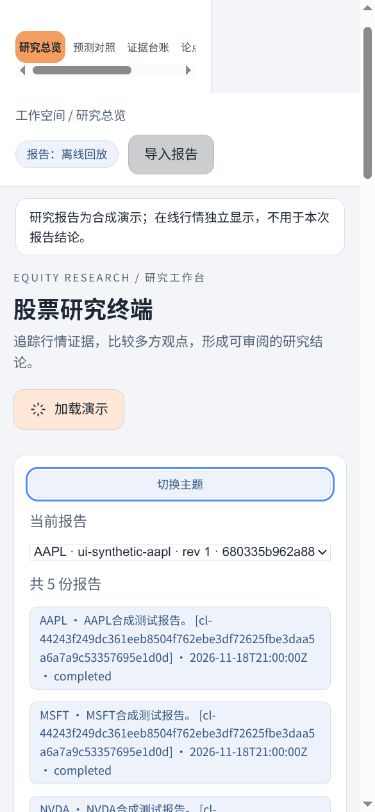
\includegraphics[height=5.0cm]{figures/phone-light.jpg}
 \end{column}
 \begin{column}{.67\textwidth}
 Real browser QA at a 390 px CSS viewport.
 \medskip
 \begin{itemize}\setlength\itemsep{7pt}
 \item Evidence inspection and explicit artifact states
 \item No page-wide horizontal overflow observed
 \item Narrow navigation remains a usability issue
 \end{itemize}
 \medskip\small\alert{Synthetic QA content. No proof of financial accuracy.}
 \end{column}
 \end{columns}
 \source{docs/verification/v0.3/screenshots/phone-light.jpg; final-review.md}
\end{frame}

\begin{frame}{Backup: evidence index}
 \small
 \begin{tabularx}{\textwidth}{@{}L{3.1cm}Y@{}}
 \toprule Topic&Local evidence\\\midrule
 Requirements&\code{requirements.yaml}, \code{Blueprint.md}\\[5pt]
 Acceptance&\code{v0.3/final-review.md}\\[5pt]
 Regression&\code{v0.3/final-review.md}, regression section\\[5pt]
 Renderer defect&\code{v0.3/structured-render-probe.txt}\\[5pt]
 Human actions&\code{pending-actions.md}\\[5pt]
 Repository&\href{https://github.com/Djangle162857/evidenceguard-tradingagents-cs5351/tree/codex/evidenceguard-candidate}{EvidenceGuard candidate on GitHub}\\\bottomrule
 \end{tabularx}
 \medskip\small Consult GitHub Actions for candidate check results and current branch status.
 \source{docs/verification/v0.3/final-review.md and docs/code-governance/github-evidence.md}
\end{frame}
\end{document}
